\documentclass{article}

\usepackage[dblblindworkshop, final, nonatbib]{neurips_2026}
\workshoptitle{Second Workshop on Large Language Models for Social Reasoning and Simulation}

\usepackage[utf8]{inputenc}
\usepackage[T1]{fontenc}
\usepackage{hyperref}
\usepackage{url}
\usepackage{booktabs}
\usepackage{microtype}
\usepackage{graphicx}
\usepackage{tikz}
\usetikzlibrary{arrows.meta, positioning, calc}
\usepackage{array}
\usepackage{xcolor}

\title{Beyond Believability: Evidence-Linked Context\\Representations for Behaviourally Grounded Social Agents}

\author{%
  Roki Seydi \\
  University College London \\
  \texttt{roki.seydi.26@ucl.ac.uk}
}

\begin{document}

\maketitle

\begin{abstract}
Social agents can sound human without reconstructing the humans they represent.
We test whether an evidence-linked relational-behaviour graph, alone or combined
with memory and reflection, improves grounded reconstruction over a compact
persona or memory alone. From approximately 230 minutes of edited couples-therapy
material, we build representations from earlier episodes and evaluate 400
condition-blind predictions for 5 participants on later held-out situations. Three
architectures lead for different participants in this small sample; the hybrid never
ranks first, and mechanistic fidelity diverges from observable fidelity. Graphs
support provenance and explicit conditional pathways, but errors increase when
meaning is carried by surrounding partners or non-verbal behaviour omitted from
transcripts. These preliminary findings point toward evidence-calibrated
combinations of memory, structured mechanisms and multimodal evidence for
behaviourally grounded, psychologically plausible agents. The relevant question is
not which persona is most convincing, but which evidence and representation are
adequate for the inference being made.
\end{abstract}

\section{Introduction}

Believability is a common success criterion for social agents, but it does not establish fidelity to
the target. A fluent response may be reasonable in general yet unsupported by the target's history,
relationships or observed actions~\cite{wang2025llm,wu2025boundary,lu2025llm}. This gap matters when agents stand in for
real people or are aggregated into simulated populations: individually plausible errors can change
interactions and downstream conclusions.

We ask a simple empirical question: \textit{what kind of context helps an LLM reconstruct a person's
later behaviour?} We compare a compact persona, chronological memory with reflection, an
evidence-linked behavioural graph, and a memory--graph hybrid. Rather than asking whether an
output merely ``sounds right'', we hide a later observed response and score whether the model
recovers its interpretation, affect, objective, action, escalation or repair, and immediate effect on
a partner.

The distinction is between \textit{psychological plausibility}---a defensible account of why someone
might respond---and \textit{behavioural grounding}---evidence that this person responded in this way.
Achieving behavioural grounding depends on the evidence available to the agent and how that
evidence is represented. A prediction may fail because the representation obscures an important
mechanism, or because the source material never captured the decisive signal. Adding more text
cannot recover omitted gaze, posture, prosody, silence, timing or relationships; yet providing too
little evidence can invite generic assumptions.

We contribute (i)~a provenance-aware relational-behaviour graph---a structured map connecting a
person's history and situations to interpretations, affect, relational objectives, behaviour and partner
effects, with each connection tied to its source and uncertainty---(ii)~a temporal holdout protocol
separating mechanistic from observable fidelity, and (iii)~an empirical comparison that, within this
small sample, complicates our initial expectation that the hybrid would be strongest. Different
representations lead for different participants, and richer context sometimes supports a persuasive
but wrong story. The result reframes context design as an evidence-selection problem rather than a
contest to build the most elaborate persona.

This proof-of-concept methodology proposal establishes these three tools and surfaces questions---
architecture heterogeneity, the mechanistic--observable gap and missing modalities---for larger
multimodal evaluation. Its participant-level results suggest that meaningful capture of human
behaviour is conditional on the person and available evidence, not a fixed property of an
architecture.

\section{Related work}

Behavioural science motivates longitudinal representation: past behaviour can inform future
behaviour through repeated routines and intentions, while personality research locates consistency
in situation-dependent ``if--then'' signatures rather than static traits~\cite{ouellette1998habit,mischel1995cognitive}.
Generative Agents established memory and reflection as a basis for believable agents~\cite{park2023generative};
subsequent work grounds agents in interviews, behavioural histories and psychological
patterns~\cite{park2024generative,li2025digital,wang2026humanllm}. Persona and graph-based approaches add
structure~\cite{meng2026psyagent,qi2026dynamic,liang2025personaagent}, but do not generally retain the provenance,
evidential status, competing explanations and revisions behind each behavioural link. Our graph
treats those features as part of the representation, making situation--mechanism--behaviour
pathways inspectable. We test whether that auditability also improves held-out reconstruction,
alone or with memory, while prior evaluations show weak prompt-only alignment with observed
behaviour~\cite{hoang2026llms,wang2025llm,lu2025llm}.

\section{Evidence-linked context representations}

\paragraph{Source and construction.}
The source comprises nine approximately 26-minute episodes (about 230 minutes) from Season~4
of \textit{Couples Therapy}, following nine participants across four relationship systems~\cite{kriegman2024couples}.
This is a useful stress test because the same people return across time, describe their own motives,
respond to partners, receive competing interpretations and sometimes revise earlier accounts. It
therefore supports both longitudinal evidence construction and a genuine later holdout, while making
relational errors visible: predicting one person often requires understanding what another person
did or meant. AI-assisted transcription and preliminary structuring were followed by human speaker
correction and longitudinal cross-checking. We retain individual accounts alongside relationship-level
overlap and disagreement, adapting dyadic Framework analysis~\cite{collaco2021framework}. The programme is
edited and performative, not diagnostic truth.

A behavioural pathway connects context, situation, appraisal, internal state, behaviour and partner
effect (Figure~\ref{fig:main}a). Missing components remain missing and competing interpretations
may coexist.

\begin{figure}[t]
  \centering
  \begin{minipage}[t]{0.46\textwidth}
    \centering
    \small\textbf{a\quad Evidence-linked relational pathway}\\[6pt]
    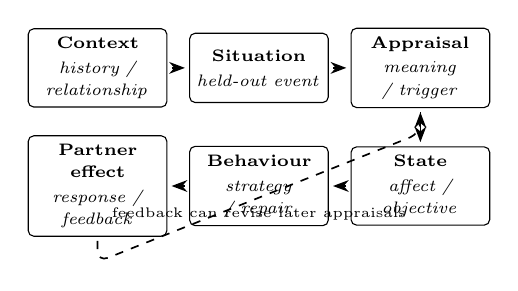
\begin{tikzpicture}[
      box/.style={draw, rounded corners=2pt, text width=1.55cm,
                  minimum height=0.88cm, align=center,
                  font=\fontsize{6.5}{8}\selectfont, inner sep=3pt},
      arr/.style={-Stealth, semithick, shorten >=1.5pt, shorten <=1.5pt}
    ]
      % Top row
      \node[box] (ctx) at (0,    1.5) {\textbf{Context}\\[1pt]
                                        \textit{history / relationship}};
      \node[box] (sit) at (2.05, 1.5) {\textbf{Situation}\\[1pt]
                                        \textit{held-out event}};
      \node[box] (app) at (4.1,  1.5) {\textbf{Appraisal}\\[1pt]
                                        \textit{meaning / trigger}};
      % Bottom row (reversed)
      \node[box] (par) at (0,    0)   {\textbf{Partner effect}\\[1pt]
                                        \textit{response / feedback}};
      \node[box] (beh) at (2.05, 0)   {\textbf{Behaviour}\\[1pt]
                                        \textit{strategy / repair}};
      \node[box] (sta) at (4.1,  0)   {\textbf{State}\\[1pt]
                                        \textit{affect / objective}};
      % Forward pathway arrows
      \draw[arr] (ctx) -- (sit);
      \draw[arr] (sit) -- (app);
      \draw[arr] (app) -- (sta);
      \draw[arr] (sta) -- (beh);
      \draw[arr] (beh) -- (par);
      % Feedback (dashed)
      \draw[arr, dashed, rounded corners=4pt]
        (par.south) -- ++(0,-0.32)
        -- node[below, font=\fontsize{5}{6}\selectfont, align=center]
           {feedback can revise later appraisals}
        ($(app.south)+(0,-0.32)$) -- (app.south);
    \end{tikzpicture}\\[4pt]
    {\fontsize{5.5}{7}\selectfont
     Edges retain provenance, evidence status, uncertainty and alternatives.}
  \end{minipage}
  \hfill
  \begin{minipage}[t]{0.50\textwidth}
    \centering
    \small\textbf{b\quad Mean fidelity (/12): no universal winner}\\[6pt]
    \fontsize{7.5}{9}\selectfont
    \begin{tabular}{lrrrrrr}
      \toprule
               & \textbf{A} & \textbf{B} & \textbf{C} & \textbf{D} & \textbf{E} & \textbf{Pooled} \\
      \midrule
      Minimal  & 7.55 & 6.85 & \textbf{6.75} & 4.10 & \textbf{6.25} & \textbf{6.30} \\
      Memory   & \textbf{8.65} & 6.85 & 5.00 & 2.70 & 5.15 & 5.67 \\
      Graph    & 7.75 & \textbf{7.25} & 5.70 & \textbf{4.40} & 5.70 & 6.16 \\
      Hybrid   & 8.00 & 6.80 & 5.30 & 2.30 & 6.00 & 5.68 \\
      \bottomrule
    \end{tabular}
  \end{minipage}
  \caption{Evidence-linked pathway (a) and mean fidelity by condition (b). Bold cells mark
    column maxima; pooled values are descriptive.}
  \label{fig:main}
\end{figure} Evidence status distinguishes direct self-report, observed behaviour, partner report,
clinical formulation, accepted formulation, recurrence and researcher inference. Demographic
membership never creates a behavioural edge without explicit source support. Immutable episode
graphs preserve what was knowable at each point; a unified graph accumulates corroboration,
contradiction and revision. This relational/systemic framing treats one partner's behaviour as
another's situation and feedback~\cite{smith1993appraisal,capozzi2025flowchart}.

\paragraph{Controlled representations.}
All conditions derive from one pre-holdout evidence set: (i)~\textbf{minimal persona}: sparse role,
relationship and explicitly stated goal information; (ii)~\textbf{memory-reflection}: chronological
observations, embedding-based retrieval, importance scoring and reflection cycles following Park
et al.~\cite{park2023generative}; (iii)~\textbf{behavioural graph}: evidence-linked conditional pathways without
the full chronology; and (iv)~\textbf{hybrid}: memory/reflections plus graph pathways. All use
gpt-5.6-luna with medium reasoning effort, identical system instructions, situation, schema and
700-token output limit. Memory retrieval uses text-embedding-ada-002. Input lengths differ
because representational form is the present ablation; matched-budget comparisons remain future
work.

\begin{table}[t]
  \caption{Held-out case: a plausible prediction adds confrontation absent from the observed
    repair-oriented response.}
  \label{tab:example}
  \centering
  \small
  \begin{tabular}{p{3.0cm} p{4.3cm} p{4.3cm}}
    \toprule
    \textbf{Situation shown to the agent} &
    \textbf{Observed response (sealed)} &
    \textbf{One blinded prediction} \\
    \midrule
    Participant E's partner could invite E to an event with another anchor partner,
    but takes no action. The missed invitation is discussed in therapy. &
    E notices that something is blocking the partner, asks how it can be resolved,
    and avoids adding anger because anger would not help. &
    E might say: ``You had the choice to include me and nothing happened.
    I feel forgotten and not genuinely considered. I need to understand why,
    and I need a clearer plan.'' \\
    \bottomrule
  \end{tabular}
\end{table}

\section{Held-out evaluation}

Episodes 1--7 provide development evidence. For each participant, four interpersonal situations
from Episodes 8--9 are frozen before the participant's interpretation or response; the remaining
situation is presented identically to each condition. The 5-participant analysis contains 20 unique
participant--situation cases across one dyad and all three differently positioned members of a
triad. Four conditions generate five repetitions per situation, yielding 80 predictions per
participant and 400 total. Repetitions estimate output variability, not independent human
observations.

Each prediction contains situation interpretation, affective stance, behavioural strategy, relational
objective, escalation/repair and immediate partner effect. Each dimension is scored 0 (mismatch),
1 (partial) or 2 (match), producing a 0--12 total. Interpretation, affect and objective form a
\textit{mechanistic} subscore (0--6); strategy, escalation and partner effect form an \textit{observable}
subscore (0--6). Outputs are shuffled and condition labels concealed. One human annotator reviews
all dimensions, starting from rubric-based proposed scores and documenting amendments. Ratings
are frozen and checksummed before the condition key is opened.

\section{Results}

In this sample, no architecture consistently dominates (Figure~\ref{fig:main}b). Memory-reflection
leads for A, the graph for B and D, and the minimal persona for C and E; the hybrid never leads.
Pooled means are 6.30 for minimal persona, 6.16 for graph, 5.68 for hybrid and 5.67 for
memory-reflection. These five-participant estimates admit sampling variability; we report no
significance tests and treat the pattern as hypothesis-generating.

Representation effects differ by dimension. Minimal persona has the highest pooled mechanistic
(3.24/6) and observable score (3.06/6), but only narrowly exceeds graph (3.20 and 2.96). For D,
minimal persona is strongest mechanistically while graph is strongest observably and overall; for E,
hybrid is marginally strongest mechanistically while minimal persona is strongest observably. Thus
a representation can generate a psychologically plausible interpretation yet predict the wrong
action, escalation or partner effect.

Situation effects are also pronounced. In E's possible-relocation case, observable fidelity is only
0.8--1.2/6 across architectures despite stronger mechanistic scores: predictions often reconstruct
surrounding partners incorrectly, while the transcript contains limited non-verbal evidence. C
likewise communicates uncertainty through visual and temporal cues incompletely preserved in
text. These cases expose a shared modality limitation rather than a failure unique to the graph.

\section{Discussion}

Three findings make the negative result informative. First, apparent representation fit varies across
participants, although five people cannot distinguish a person-by-architecture interaction from
noise. A's meanings are layered autobiographically; B's situation-to-response explanations are
comparatively explicit. Minimal persona leads for C and E, while the graph leads for B and D;
this does not establish that either representation is generally better. When decisive evidence is
missing, compact representations have fewer opportunities to elaborate the wrong mechanism.
The hybrid concatenates memory and graph without learned fusion or matched budgets, so its
result may reflect longer, unweighted context rather than a general limit of combination.

Second, plausible mechanisms and observable behaviour come apart. The minimal persona leads
both pooled subscores narrowly, yet participant-level rankings diverge: for D, it best captures
mechanism while the graph best captures observable behaviour. In the held-out example
(Table~\ref{tab:example}), the prediction recognises exclusion and a need for clarity, but turns
E's measured attempt to understand the partner into a more confrontational demand. A system
evaluated only for plausibility could count this as success; the observed strategy, escalation level
and likely partner effect say otherwise.

Third, the target is not the whole unit of prediction. C's hardest case involved an external partner
outside the focal triad; E's errors often came from assumptions about surrounding partners.
C's gaze, pauses, laughter, bodily orientation and shifts of attention were also weakly preserved
in text. Richer text could therefore become more specific without becoming better informed;
combining memory and graph did not cross this evidence boundary.

These observations suggest a selective context stack: memory for autobiographical explanation,
graphs for conditional pathways and relational position, and audiovisual models for gaze, prosody,
timing or posture. Selection must be evidence-calibrated; indiscriminate addition may multiply
unsupported inferences. The broader research claim is diagnostic: reconstruction depends on
alignment among human expression, captured evidence, represented relationships and the prediction
task. Although drawn from five individuals rather than a demographic sample, the same plausible-versus-grounded calibration applies to population-level fidelity; the mechanistic/observable split
offers one test before scaling to synthetic populations.

\section{Limitations, ethics and conclusion}

Broadcast therapy is mediated evidence, not complete lived or clinical truth. Transcripts omit or
discretise facial expression, gaze, gesture, touch, prosody, silence and interaction timing;
annotations such as ``long pause'' cannot preserve their continuous interpersonal distribution.
All conditions therefore share an information ceiling, and combining two text-derived
representations cannot recover a missing modality. Video may add evidence but remains shaped
by camera selection and editing.

The sample is purposively small because longitudinal graph construction favours depth per
participant over cast breadth. One annotator provides no inter-rater reliability estimate, and
proposed scores may anchor adjudication despite blinding. Input budgets are unmatched; the base
model may contain programme information despite neutral identifiers and contamination controls.
Therapist formulations are interpretations, and the graph adopts a relational/systemic lens.
Public availability does not remove privacy, dignity or dual-use risks~\cite{anzola2022ethics}; the method is
not diagnostic or validated for consequential decisions. We excluded cast members whose material
centred on severe trauma to avoid modelling people through their most vulnerable disclosures.

This proof of concept shows that the graph, temporal holdout and mechanistic/observable split
expose distinctions worth testing rather than settling architecture choice. Larger multimodal
studies should test whether missing-cue errors can be recovered and whether architecture
heterogeneity persists. The question is which evidence and representation support the behavioural
inference.

\begin{ack}
The author declares no competing interests.
\end{ack}

%% ---- REFERENCES ----

\begin{thebibliography}{18}

\bibitem{anzola2022ethics}
D.~Anzola, P.~Barbrook-Johnson, and N.~Gilbert.
\newblock The ethics of agent-based social simulation.
\newblock \textit{Journal of Artificial Societies and Social Simulation},
  25(4):1, 2022.
\newblock doi: 10.18564/jasss.4907.

\bibitem{capozzi2025flowchart}
F.~Capozzi.
\newblock A research-driven flowchart to approach change in couples.
\newblock \textit{Frontiers in Psychology}, 15:1438394, 2025.
\newblock doi: 10.3389/fpsyg.2024.1438394.

\bibitem{collaco2021framework}
N.~Colla{\c{c}}o, R.~Wagland, O.~Alexis, A.~Gavin, A.~Glaser, and
  E.~K.~Watson.
\newblock Using the framework method for the analysis of qualitative dyadic
  data in health research.
\newblock \textit{Qualitative Health Research}, 31(8):1555--1564, 2021.
\newblock doi: 10.1177/10497323211011599.

\bibitem{hoang2026llms}
V.~Hoang, E.~Rogers, and R.~Ross.
\newblock {LLMs} as standardised patients for motivational interviewing: How
  faithful are they?
\newblock In \textit{Proceedings of the 11th Workshop on Computational
  Linguistics and Clinical Psychology}, pages 258--270, 2026.
\newblock doi: 10.18653/v1/2026.clpsych-1.21.

\bibitem{kriegman2024couples}
J.~Kriegman, E.~Steinberg, and E.~Despres.
\newblock Couples therapy, season 4, episodes 401--409, 2024.
\newblock Executive producers; Edgeline Films and Showtime.

\bibitem{li2025digital}
R.~Li, H.~Xia, X.~Yuan, Q.~Dong, L.~Sha, W.~Li, and Z.~Sui.
\newblock How far are {LLMs} from being our digital twins? {A} benchmark for
  persona-based behavior chain simulation.
\newblock In \textit{Findings of the Association for Computational
  Linguistics: ACL 2025}, pages 15738--15763, 2025.
\newblock doi: 10.18653/v1/2025.findings-acl.813.

\bibitem{liang2025personaagent}
S.~Liang, Y.~Zhang, and Y.~Guo.
\newblock {PersonaAgent} with {GraphRAG}: Community-aware knowledge graphs for
  personalized {LLM}.
\newblock arXiv:2511.17467, 2025.

\bibitem{lu2025llm}
Y.~Lu, J.~Huang, Y.~Han, B.~Yao, S.~Bei, J.~Gesi, Y.~Xie, Y.~Sang,
  Z.~Wang, Q.~He, and D.~Wang.
\newblock Can {LLM} agents simulate multi-turn human behavior? {E}vidence from
  real online customer behavior data.
\newblock arXiv:2503.20749, 2025.
\newblock doi: 10.48550/arXiv.2503.20749.

\bibitem{meng2026psyagent}
Z.~Meng and K.~Chen.
\newblock {PsyAgent}: Constructing human-like agents based on psychological
  modeling and contextual interaction.
\newblock arXiv:2601.06158, 2026.

\bibitem{mischel1995cognitive}
W.~Mischel and Y.~Shoda.
\newblock A cognitive-affective system theory of personality: Reconceptualizing
  situations, dispositions, dynamics, and invariance in personality structure.
\newblock \textit{Psychological Review}, 102(2):246--268, 1995.
\newblock doi: 10.1037/0033-295X.102.2.246.

\bibitem{ouellette1998habit}
J.~A.~Ouellette and W.~Wood.
\newblock Habit and intention in everyday life: The multiple processes by which
  past behavior predicts future behavior.
\newblock \textit{Psychological Bulletin}, 124(1):54--74, 1998.
\newblock doi: 10.1037/0033-2909.124.1.54.

\bibitem{park2023generative}
J.~S.~Park, J.~O'Brien, C.~J.~Cai, M.~R.~Morris, P.~Liang, and
  M.~S.~Bernstein.
\newblock Generative agents: Interactive simulacra of human behavior.
\newblock In \textit{UIST}, 2023.
\newblock doi: 10.1145/3586183.3606763.

\bibitem{park2024generative}
J.~S.~Park, C.~Q.~Zou, A.~Shaw, B.~M.~Hill, C.~Cai, M.~R.~Morris,
  R.~Willer, P.~Liang, and M.~S.~Bernstein.
\newblock Generative agent simulations of 1,000 people.
\newblock arXiv:2411.10109, 2024.
\newblock doi: 10.48550/arXiv.2411.10109.

\bibitem{qi2026dynamic}
Y.~Qi, X.~Zhang, R.~Zeng, M.~Liu, Z.~Zhou, D.~Miao, B.~Yan, and Z.~Guan.
\newblock Beyond static persona consistency: Dynamic persona coherence in
  {LLM} role-playing.
\newblock In \textit{Proceedings of the 64th Annual Meeting of the Association
  for Computational Linguistics}, pages 28942--28956, 2026.
\newblock doi: 10.18653/v1/2026.acl-long.1336.

\bibitem{smith1993appraisal}
C.~A.~Smith and R.~S.~Lazarus.
\newblock Appraisal components, core relational themes, and the emotions.
\newblock \textit{Cognition and Emotion}, 7(3--4):233--269, 1993.
\newblock doi: 10.1080/02699939308409189.

\bibitem{wang2025llm}
Q.~Wang, J.~Wu, Z.~Jiang, Z.~Tang, B.~Luo, N.~Chen, W.~Chen, H.~Wang, and
  B.~He.
\newblock {LLM}-based human simulations have not yet been reliable.
\newblock arXiv:2501.08579, 2025.
\newblock doi: 10.48550/arXiv.2501.08579.

\bibitem{wang2026humanllm}
X.~Wang, J.~Yang, W.~Li, R.~Xie, J.~Huang, J.~Gao, S.~Huang, Y.~Kang,
  Y.~Guo, H.~Feng, and Y.~Xiao.
\newblock {HumanLLM}: Benchmarking and improving {LLM} anthropomorphism via
  human cognitive patterns.
\newblock In \textit{Proceedings of the 64th Annual Meeting of the Association
  for Computational Linguistics}, pages 38486--38517, 2026.
\newblock doi: 10.18653/v1/2026.acl-long.1783.

\bibitem{wu2025boundary}
Z.~Wu, R.~Peng, T.~Ito, M.~Onizuka, and C.~Xiao.
\newblock {LLM}-based social simulations require a boundary.
\newblock arXiv:2506.19806, 2025.

\end{thebibliography}

%% ---- APPENDICES ----

\appendix

\section{Reproducibility materials}

Code, representations, protocols and experimental artefacts are available at
\url{https://github.com/rokiseydi/beyond-believability}.
% TODO before submission: create this repo and verify the URL is live
The repository contains the evidence-status codebook; canonical pre-holdout evidence tables;
the four representation packages with token counts; prompts, model identifiers, seeds and
generation parameters; all blinded outputs; frozen human-adjudicated ratings and checksums;
blinding keys; scoring rubric; additional graph figures; and episode provenance. Blinding keys
are provided for audit but were not opened until ratings were frozen.

\section{Evidence status and scope}

Edges are labelled as direct self-report, observed behaviour, partner report, clinical formulation,
accepted formulation, repeated observation, literature-supported hypothesis or researcher
inference. Alternative pathways are retained where evidence conflicts. No edge is created from
demographic membership alone. Future work should use consented multimodal longitudinal data,
participant review, multiple annotators, matched-budget ablations and explicit governance for
access to high-fidelity behavioural agents.

\end{document}
